\section*{Results}

\subsection*{Qualitative Observations}

The current going through the wire fluctuated as the wire swung, likely due to the changing contact of the wire with the supports.
There were specific ranges where the current would fluctuate, mainly at the lower currents.
At around $1.40\si{\ampere}$, the wire would get close enough to the bracket that it would jump and stick to the bracket.
This was mitigated by avoiding current from exceeding $1.50\si{\ampere}$.
From visual observation, the angle of deflection would increase as the current increased, but their relationship was determinable
from visuals.

\subsection*{Raw Data}

The data provided below shows the measured current and respective measured angle from 5 trials.
The angle measurements were done through the measurement tool in GIMP.

\begin{table}[H]
	\centering
	\onehalfspacing
	\begin{tabular}{|lr||lr||lr||lr||lr|}
		\hline
		\multicolumn{2}{|c||}{Trial 1} & \multicolumn{2}{|c||}{Trial 2} & \multicolumn{2}{c||}{Trial 3}& \multicolumn{2}{c||}{Trial 4}& \multicolumn{2}{c|}{Trial 5} \\
		\hline
		$I(\si{\ampere})$ & $\theta(\si{\degree})$ & $I(\si{\ampere})$ & $\theta(\si{\degree})$ & $I(\si{\ampere})$ & $\theta(\si{\degree})$ & $I(\si{\ampere})$ & $\theta(\si{\degree})$ & $I(\si{\ampere})$ & $\theta(\si{\degree})$ \\
		$\pm0.01$ & $\pm0.01$ & $\pm0.01$ & $\pm0.01$ & $\pm0.01$ & $\pm0.01$ & $\pm0.01$ & $\pm0.01$ & $\pm0.01$ & $\pm0.01$ \\
		\hline
		0 & 0.62 & 0 & 0.48 & 0 & 0.57 & 0 & 0.57 & 0 & 0.66 \\
		0.22 & 5.53 & 0.23 & 6.83 & 0.26 & 6.62 & 0.18 & 4.11 & 0.19 & 4.37 \\
		0.39 & 12.02 & 0.42 & 12.63 & 0.46 & 13.65 & 0.39 & 11.3 & 0.44 & 13.25 \\
		0.58 & 17.41 & 0.59 & 17.78 & 0.57 & 16.88 & 0.61 & 17.82 & 0.61 & 18.14 \\
		0.80 & 22.02 & 0.88 & 23.49 & 0.78 & 21.65 & 0.83 & 22.64 & 0.82 & 22.35 \\
		1.04 & 25.84 & 1.01 & 25.51 & 1.01 & 25.47 & 1.06 & 25.98 & 0.99 & 25.05 \\
		1.20 & 28.59 & 1.21 & 27.82 & 1.20 & 28.29 & 1.22 & 28.44 & 1.18 & 27.78 \\
		1.42 & 31.65 & 1.40 & 30.84 & 1.41 & 31.23 & 1.42 & 30.93 & 1.38 & 30.41 \\
		\hline
	\end{tabular}
	\caption{Raw data table of measured angles $\theta$ for increasing values of $I$ over 5 trials.}
	\label{tab:raw1}
\end{table}

\newpage

\subsection*{Processed Data}

To account for a potential offset in angle due to the shape of the wire, the measured angle of the wire at rest is subtracted from all other measurements.
This was calculated as:
\begin{equation*}
	\theta_{\text{final}} = \theta_{\text{measured}} - \theta_0 \text{.}
\end{equation*}
For example, the for the first data point, $5.53\si{\degree} - 0.62\si{\degree} = 4.91\si{\degree}$.
The uncertainty of the measured angle was propagated as such:
\begin{equation*}
	\Delta\theta_{\text{final}} = \Delta\theta_{\text{measured}} + \Delta\theta_0 \text{.}
\end{equation*}
For the first data point, $\pm(0.01 + 0.01)\si{\degree} = \pm0.02\si{\degree}$.
This was done for each trial.

The average deflection angle for each target current (ie. $0.20\si{\ampere}$, $0.40\si{\ampere}$, etc.) will not be taken, given the inherent variation of current.

\begin{table}[H]
	\centering
	\onehalfspacing
	\begin{tabular}{|lr||lr||lr||lr||lr|}
		\hline
		\multicolumn{2}{|c||}{Trial 1} & \multicolumn{2}{|c||}{Trial 2} & \multicolumn{2}{c||}{Trial 3}& \multicolumn{2}{c||}{Trial 4}& \multicolumn{2}{c|}{Trial 5} \\
		\hline
		$I(\si{\ampere})$ & $\theta(\si{\degree})$ & $I(\si{\ampere})$ & $\theta(\si{\degree})$ & $I(\si{\ampere})$ & $\theta(\si{\degree})$ & $I(\si{\ampere})$ & $\theta(\si{\degree})$ & $I(\si{\ampere})$ & $\theta(\si{\degree})$ \\
		$\pm0.01$ & $\pm0.02$ & $\pm0.01$ & $\pm0.02$ & $\pm0.01$ & $\pm0.02$ & $\pm0.01$ & $\pm0.02$ & $\pm0.01$ & $\pm0.02$ \\
		\hline
		0.22 & 4.91 & 0.23 & 6.35 & 0.26 & 6.05 & 0.18 & 3.54 & 0.19 & 3.71 \\
		0.39 & 11.40 & 0.42 & 12.15 & 0.46 & 13.08 & 0.39 & 10.73 & 0.44 & 12.59 \\
		0.58 & 16.79 & 0.59 & 17.30 & 0.57 & 16.31 & 0.61 & 17.25 & 0.61 & 17.48 \\
		0.80 & 21.40 & 0.88 & 23.01 & 0.78 & 21.08 & 0.83 & 22.07 & 0.82 & 21.69 \\
		1.04 & 25.22 & 1.01 & 25.03 & 1.01 & 24.90 & 1.06 & 25.41 & 0.99 & 24.39 \\
		1.20 & 27.97 & 1.21 & 27.34 & 1.20 & 27.72 & 1.22 & 27.87 & 1.18 & 27.12 \\
		1.42 & 31.03 & 1.40 & 30.36 & 1.41 & 30.66 & 1.42 & 30.36 & 1.38 & 29.75 \\
		\hline
	\end{tabular}
	\caption{Corrected angle data table for measured angles $\theta$.}
	\vspace{-10pt}
	\label{tab:raw2}
\end{table}

The data in Table \ref{tab:raw2} is plotted in Figure \ref{fig:rawplot}.

Next, the corrected angle data was used to calculate the force exerted on the wire. This was calculated as:
\begin{equation*}
	F = mg \tan\theta
\end{equation*}
where $m = 4.9\pm0.1\si{\gram}$ and $g = 9.81\si{\meter\per\second\squared}$.

\begin{figure}[H]
	\centering
	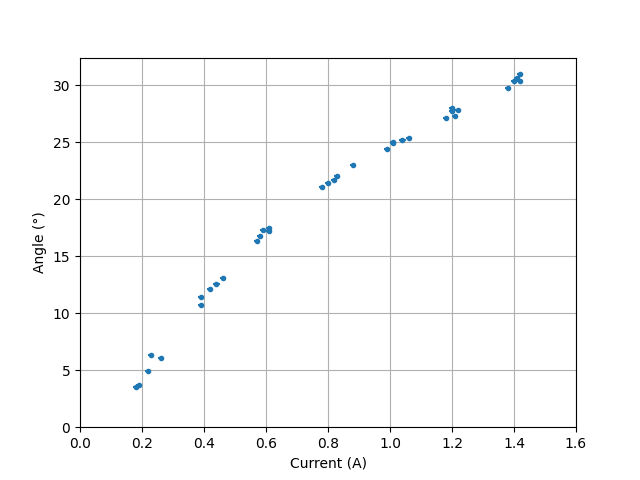
\includegraphics[width=0.8\textwidth]{figures/rawplot.png}
	\caption{Plot of corrected measured angles vs current. Note that the errorbars are so small that they are barely visible in the graph}
	\label{fig:rawplot}
\end{figure}
